\section{Two symmetric weighted \texorpdfstring{$K_4$}{K4} families}\label{app:k4}

Let $G_{13}(x)$ have one core vertex, three satellites, unit
core--satellite weights, and satellite--satellite weight $x>0$.  Let
$G_{22}(x,y)$ have two vertex pairs, internal-pair weights $x,y>0$, and four
unit cross-pair weights.  These are the full $S_1\times S_3$ and
$S_2\times S_2$ invariant families after common scaling.

\begin{figure}[H]
\centering
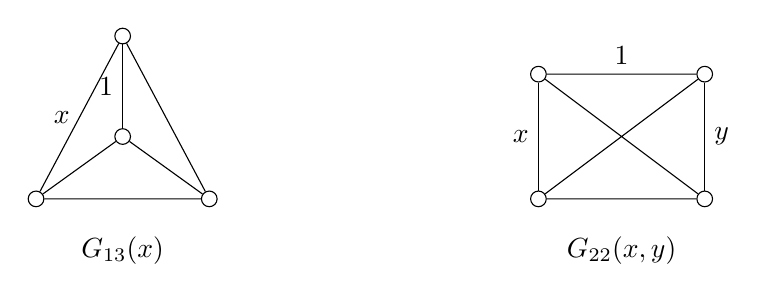
\begin{tikzpicture}[vertex/.style={circle,draw,fill=white,inner sep=2pt},scale=.88]
  \begin{scope}[xshift=-3.6cm]
    \node[vertex] (c) at (0,0) {};
    \node[vertex] (a) at (0,1.45) {};
    \node[vertex] (b) at (-1.25,-.9) {};
    \node[vertex] (d) at (1.25,-.9) {};
    \draw (c)--node[left] {$1$}(a); \draw (c)--(b) (c)--(d);
    \draw (a)--node[left] {$x$}(b)--(d)--(a);
    \node at (0,-1.65) {$G_{13}(x)$};
  \end{scope}
  \begin{scope}[xshift=3.6cm]
    \node[vertex] (a1) at (-1.2,.9) {};
    \node[vertex] (a2) at (-1.2,-.9) {};
    \node[vertex] (b1) at (1.2,.9) {};
    \node[vertex] (b2) at (1.2,-.9) {};
    \draw (a1)--node[left] {$x$}(a2);
    \draw (b1)--node[right] {$y$}(b2);
    \draw (a1)--node[above] {$1$}(b1) (a1)--(b2)
          (a2)--(b1) (a2)--(b2);
    \node at (0,-1.65) {$G_{22}(x,y)$};
  \end{scope}
\end{tikzpicture}
\caption{The two invariant weighted $K_4$ families.  Unlabeled edges have
unit weight.}
\label{fig:k4}
\end{figure}

A two-class graph with class sizes $p,q$, internal weights $\alpha,\beta$,
and cross weight $\gamma$ is strongly lumpable by mutant counts $(i,j)$.
The four state-changing probabilities follow directly from \eqref{2.2}:
\begin{align}
 P_{i,j}^{i+1,j}
 &=\frac{p-i}{p+q}\frac{r(i\alpha+j\gamma)}
 {r(i\alpha+j\gamma)+(p-i-1)\alpha+(q-j)\gamma},\notag\\
 P_{i,j}^{i-1,j}
 &=\frac{i}{p+q}\frac{(p-i)\alpha+(q-j)\gamma}
 {r((i-1)\alpha+j\gamma)+(p-i)\alpha+(q-j)\gamma},\notag\\
 P_{i,j}^{i,j+1}
 &=\frac{q-j}{p+q}\frac{r(j\beta+i\gamma)}
 {r(j\beta+i\gamma)+(q-j-1)\beta+(p-i)\gamma},\notag\\
 P_{i,j}^{i,j-1}
 &=\frac{j}{p+q}\frac{(q-j)\beta+(p-i)\gamma}
 {r((j-1)\beta+i\gamma)+(q-j)\beta+(p-i)\gamma}.
                                                               \tag{B.1}\label{B.1}
\end{align}

For the $1+3$ family, exact elimination gives
\[
 \rho_{\dB}(G_{13}(x),r)-\rho_{\dB}(J_4,r)
 =-\frac{3r^2(r-1)(x-1)^2F_{13}}
 {4(r^2+r+1)P_{13}},                                       \tag{B.2}\label{B.2}
\]
where
\[
\begin{aligned}
F_{13}={}&2r^4x^2+2r^4x+11r^3x^2+14r^3x+3r^3
 +21r^2x^2+29r^2x+12r^2\\
&+16rx^2+22rx+8r+4x^2+5x+1,
\end{aligned}
\]
and
\[
\begin{aligned}
P_{13}={}&8x^2(x+1)(r^6+1)
 +(6x^4+36x^3+46x^2+16x)(r^5+r)\\
&+(27x^4+73x^3+85x^2+59x+12)(r^4+r^2)\\
&+(42x^4+90x^3+106x^2+66x+24)r^3.
\end{aligned}
\]
Every coefficient is positive.

For the $2+2$ family,
\[
 \rho_{\dB}(G_{22}(x,y),r)-\rho_{\dB}(J_4,r)
 =-\frac{r^2(r-1)H_{22}(x,y,r)}
 {4(r^2+r+1)P_{22}(x,y,r)}.                                 \tag{B.3}\label{B.3}
\]
The reduced $P_{22}$ has 123 positive integer monomials.  Independently,
the holding-step-free transient matrix $M_{22}$ satisfies
\[
 \det M_{22}=\frac{P_{22}}{128L_{22}},                       \tag{B.4}\label{B.4}
\]
where
\[
\begin{aligned}
L_{22}={}&(2r+x)(2r+y)(rx+2)(ry+2)(r+x+1)(r+y+1)\\
&\times(rx+r+1)(ry+r+1)>0.
\end{aligned}
\]
Absorption makes $M_{22}$ a nonsingular $M$-matrix, so $P_{22}>0$.

Set $g=\sqrt{xy}>0$, $d=(\sqrt x-\sqrt y)^2\ge0$, and $t=r-1>0$.
Then
\[
 H_{22}=C_0(g,t)+C_1(g,t)d+C_2(g,t)d^2+C_3(g,t)d^3+C_4(g,t)d^4. \tag{B.5}\label{B.5}
\]
Here
\[
 C_0=2t(g-1)^2(g+1)(t+1)R_0,
\]
\[
\begin{aligned}
R_0={}&(2g^2+2g)t^4+(g^3+10g^2+21g+6)t^3\\
&+(3g^3+26g^2+61g+38)t^2+(4g^3+32g^2+80g+64)t\\
&+2g^3+16g^2+40g+32,
\end{aligned}
\]
and
\[
\begin{aligned}
C_1={}&2(g^4+4g^3-2g^2+4g+1)t^6
 +(11g^4+108g^3+76g^2+60g+17)t^5\\
&+2(40g^4+288g^3+393g^2+176g+19)t^4\\
&+(16g^5+331g^4+1704g^3+2766g^2+1360g+39)t^3\\
&+2(28g^5+337g^4+1426g^3+2399g^2+1378g+12)t^2\\
&+2(g+2)(32g^4+263g^3+722g^2+661g+2)t\\
&+24g(g+2)(g+4)(g^2+4g+5),\\[2pt]
C_2={}&2(g^2+1)t^6+3(9g^2+26g+5)t^5
 +2(18g^3+120g^2+321g+44)t^4\\
&+2(2g^4+105g^3+525g^2+1071g+170)t^3\\
&+(14g^4+474g^3+2201g^2+3648g+689)t^2\\
&+2(8g^4+240g^3+1080g^2+1587g+331)t\\
&+6(g^4+30g^3+133g^2+186g+40),\\[2pt]
C_3={}&13t^5+(6g^2+48g+107)t^4+(35g^2+312g+357)t^3\\
&+(79g^2+744g+608)t^2+(80g^2+768g+529)t
 +6(5g^2+48g+31),\\
C_4={}&6t^4+39t^3+93t^2+96t+36.
\end{aligned}
\]
Every displayed coefficient is positive except for the single grouped factor
\[
 g^4+4g^3-2g^2+4g+1=(g^2-1)^2+4g(g^2+1)>0.                  \tag{B.6}\label{B.6}
\]
Thus $C_j>0$ for $j\ge1$ and $C_0\ge0$.  If $d>0$, then $C_1d>0$; if $d=0$,
$H_{22}=C_0$ vanishes only at $g=1$.

\begin{theorem}[symmetric weighted $K_4$ families]\label{thm:k4}
For every $r>1$,
\[
 \rho_{\dB}(G_{13}(x),r)\le\rho_{\dB}(J_4,r),\qquad
 \rho_{\dB}(G_{22}(x,y),r)\le\rho_{\dB}(J_4,r).
\]
Equality holds only at $x=1$ in the first family and $x=y=1$ in the second.
\end{theorem}

This is not a classification of the unrestricted six-edge weighted $K_4$.
